\documentclass{article}
\usepackage[utf8]{inputenc}
\usepackage[english]{babel}
\usepackage{amsmath}
\usepackage{graphicx}
\usepackage{hyperref}
\usepackage{caption}

\begin{document}

{\centering

\rule{\textwidth}{1.6pt}\vspace*{-\baselineskip}\vspace*{2pt} 
\rule{\textwidth}{0.4pt}\\[\baselineskip] 
{\LARGE Growing Degree Day}
\rule{\textwidth}{0.4pt}\vspace*{-\baselineskip}\vspace{3.2pt}
\rule{\textwidth}{1.6pt}\\[\baselineskip] 

\vspace{20mm} %5mm vertical space
\scshape % Small caps
CMSC 6950 - Computer Based Research Tools and Applications \\ [\baselineskip]
Project Report \\[\baselineskip]
\vspace{20mm} %5mm vertical space
Submitted by \\[\baselineskip]
{\Large Dawei Wang \\ Ajay Vijayakumar \\ Demarey Baker \\ Haqqani Gulam\par}
\vfill
{\itshape Memorial University of Newfoundland \\ St. John's, Canada.\par} 
}

\newpage



\section{ \bf Introduction}
For this project, we have selected three cities from Canada, namely: Halifax, Ottawa and Calgary, for which we calculated and visually analysed the growing degree days for years 2016 and 2017.

\section{ \bf Core Tasks}
The weather data was downloaded for the three cities and different plots were generated after calculating the GDD for those cities.

\subsection{Min/Max Plots}

\subsubsection{HALIFAX}

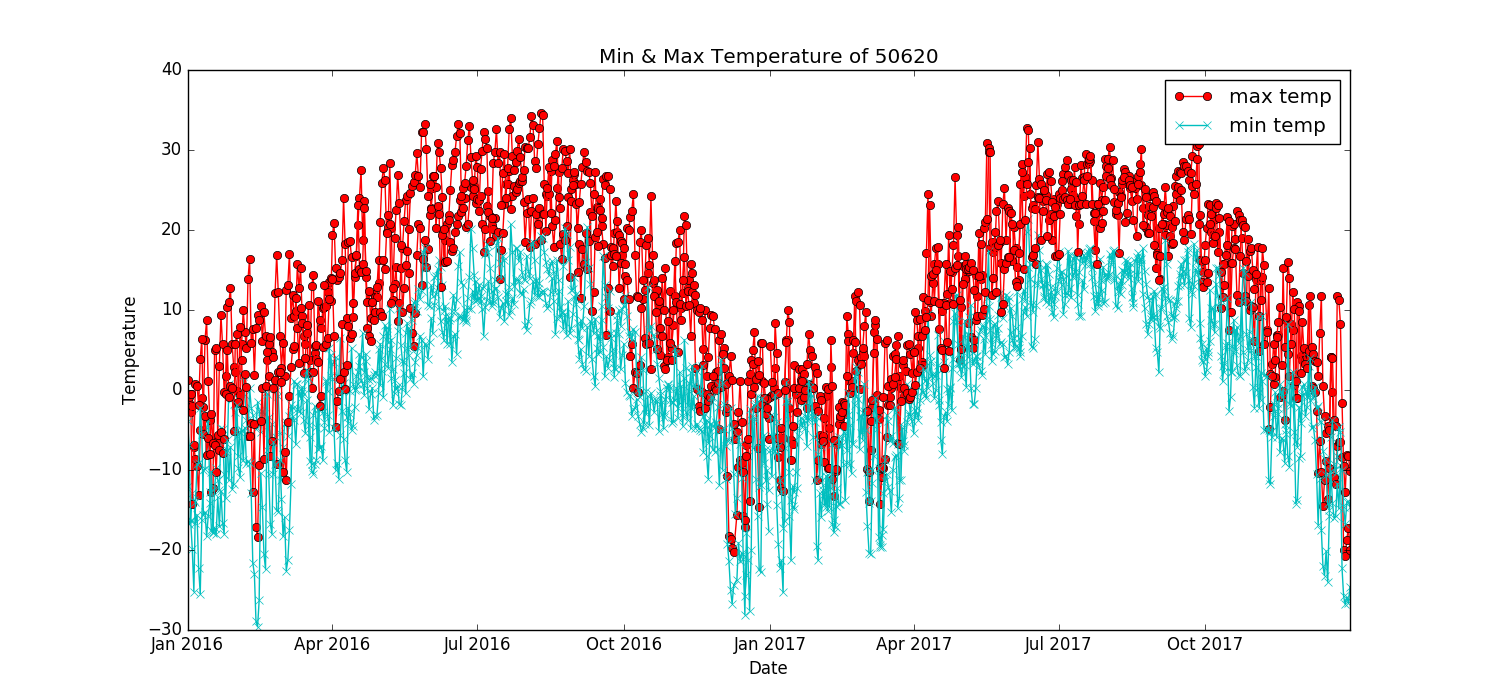
\includegraphics[scale=0.35]{./Plots/50620-2017_minmax.png}\\

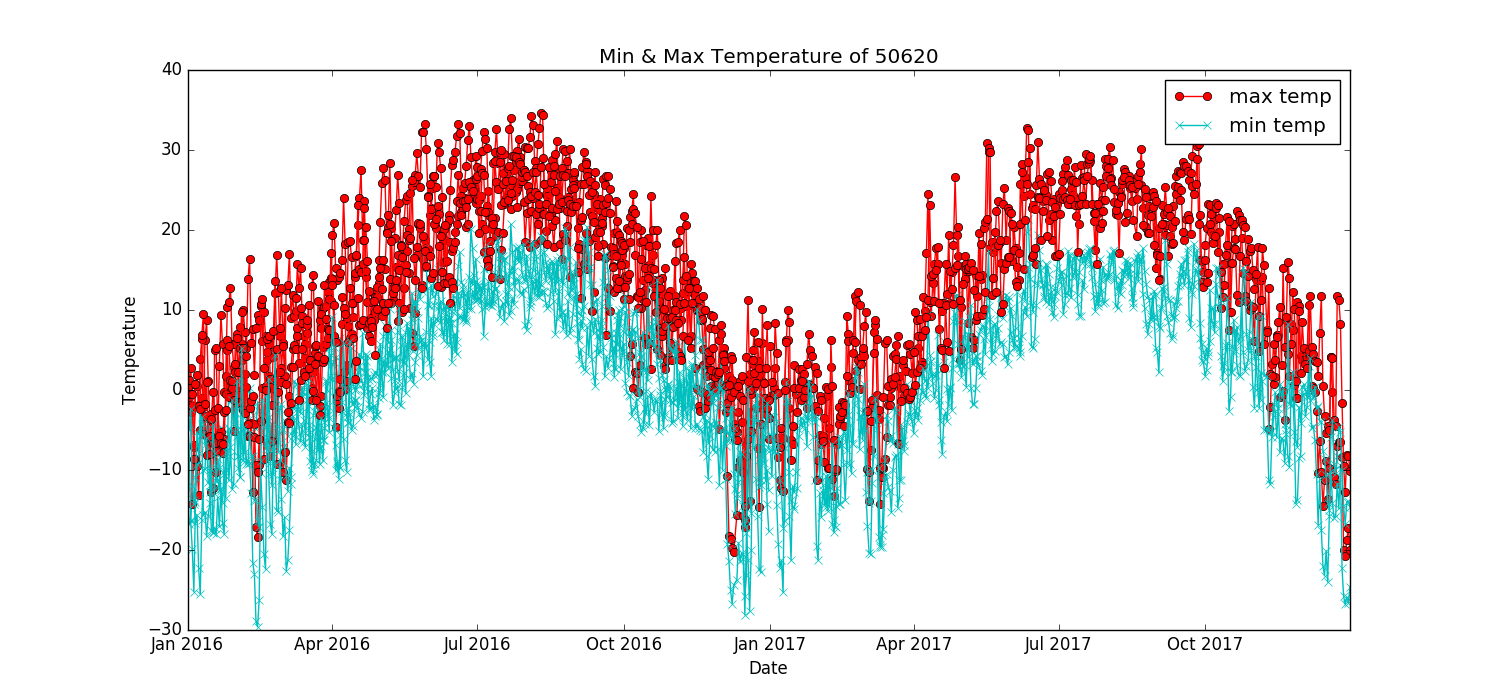
\includegraphics[scale=0.35]{./Plots/50620-2016_minmax.png}\\

\subsubsection{CALGARY}

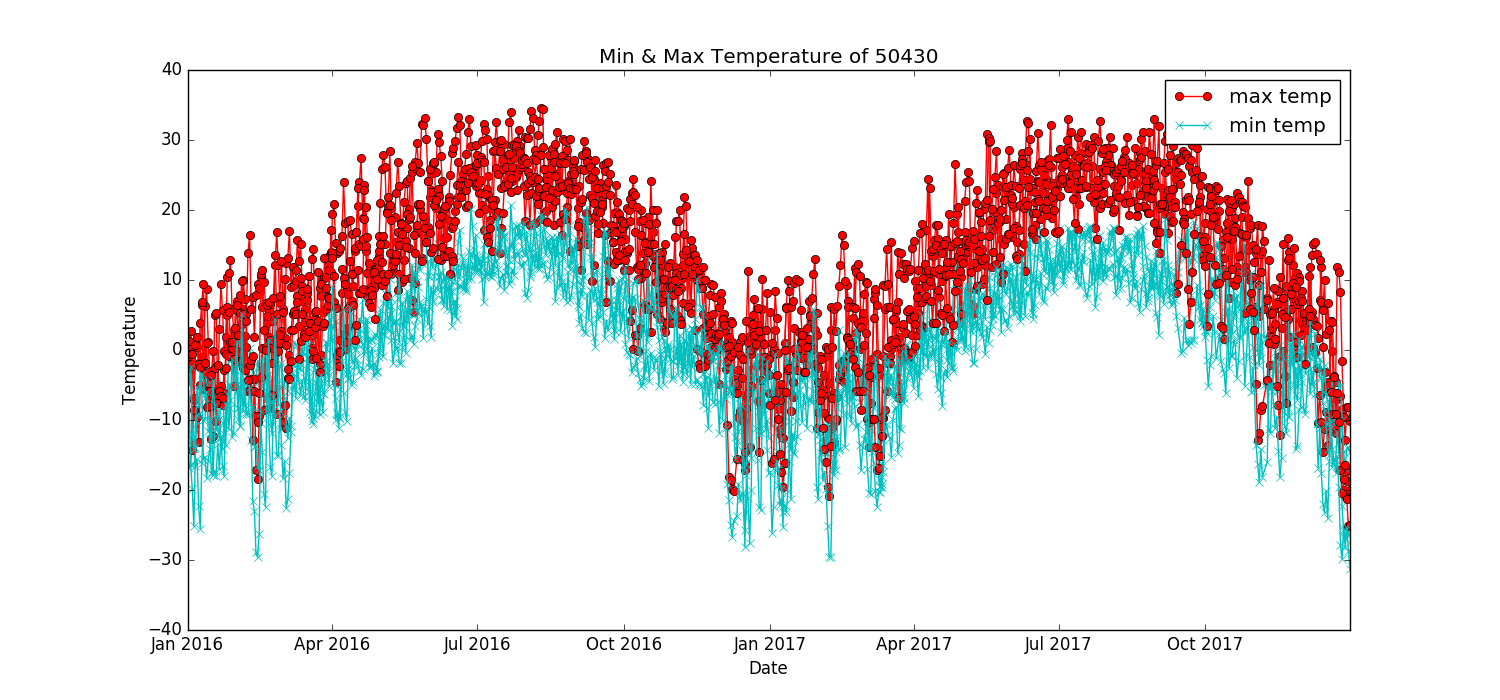
\includegraphics[scale=0.35]{./Plots/50430-2017_minmax.png}\\

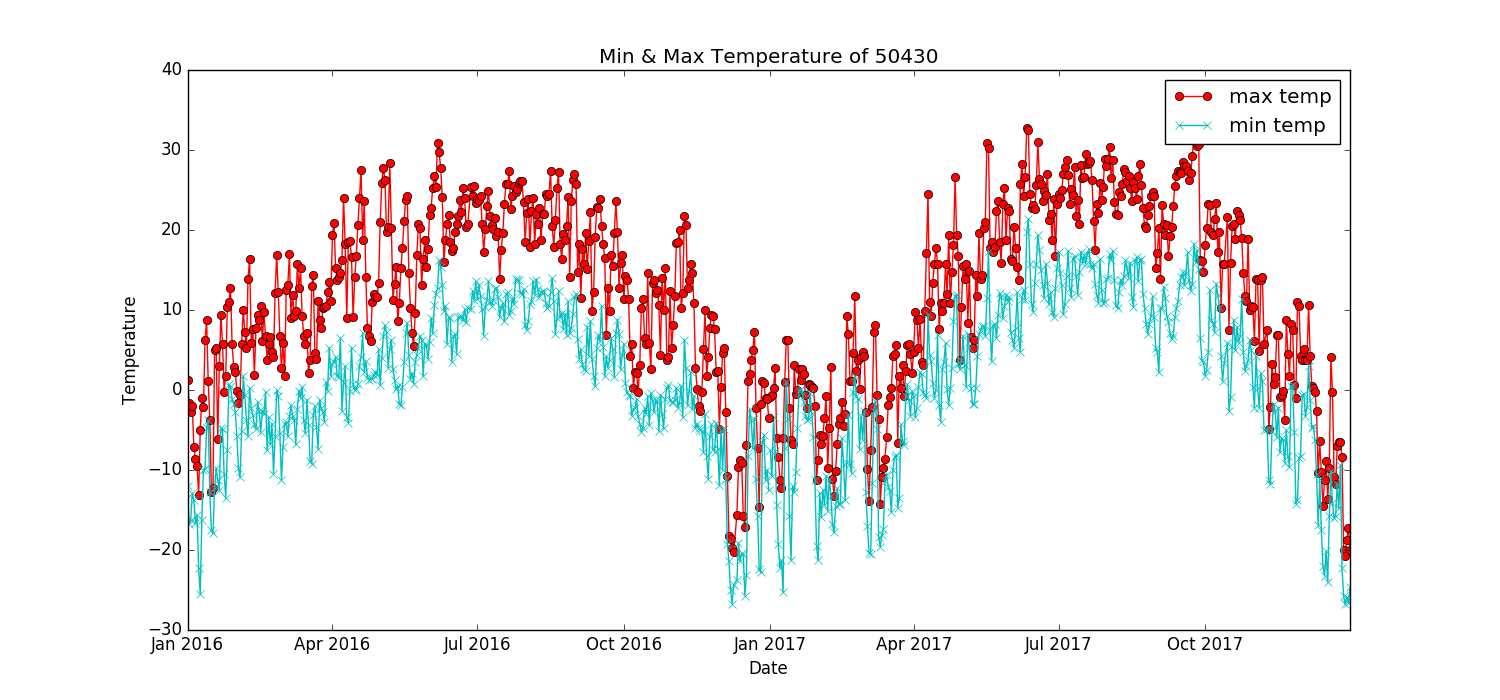
\includegraphics[scale=0.35]{./Plots/50430-2016_minmax.png}\\

\subsubsection{OTTAWA}

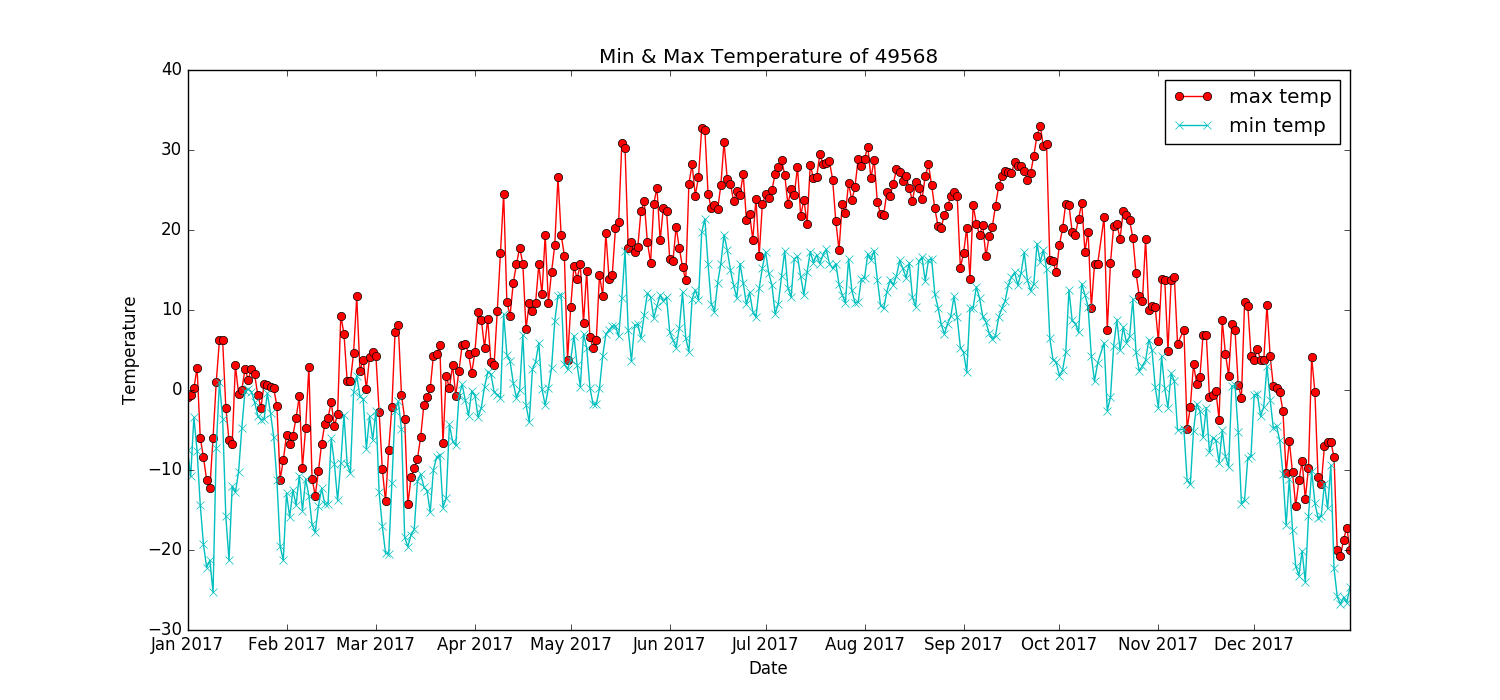
\includegraphics[scale=0.35]{./Plots/49568-2017_minmax.png}\\

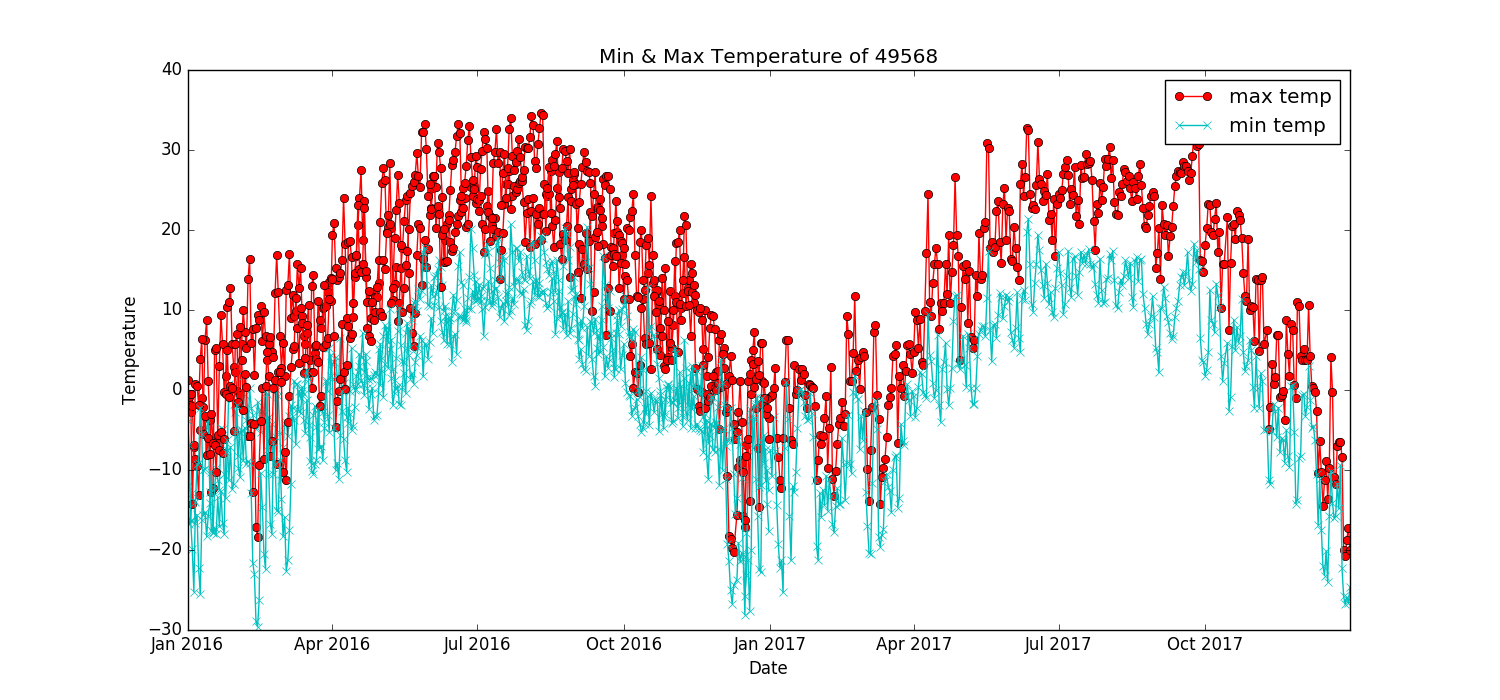
\includegraphics[scale=0.35]{./Plots/49568-2016_minmax.png}\\

\subsection{Cummulative GDD}

\includegraphics[scale=0.55]{./Plots/"HALIFAX INTL A".png}\\

\includegraphics[scale=0.55]{./Plots/"CALGARY INTL A".png}\\

\includegraphics[scale=0.55]{./Plots/"OTTAWA INTL A".png}\\

\section{ \bf Core Tasks}
\subsection{GDD with varying Base Temperature}

\subsubsection{OTTAWA}

\includegraphics[scale=0.55]{./docs/plots/49568_daily_gdd_plot.png}\\

\subsubsection{HALIFAX}

\includegraphics[scale=0.55]{./docs/plots/50620_daily_gdd_plot.png}\\

\subsubsection{CALGARY}

\includegraphics[scale=0.55]{./docs/plots/50430_daily_gdd_plot.png}\\


\subsection{Effective growing degree days of Newfoundland in 2015}

\includegraphics[scale=0.55]{./docs/plots/GDD_Map_NL.png}\\

\subsection{Effective growing degree days of Canada in 2016}

\includegraphics[scale=0.55]{./docs/plots/GDD_Map_CAN_scatter.png}\\

\includegraphics[scale=0.55]{./docs/plots/GDD_Map_CAN_contour.png}\\


\section{Conclusion}



\end{document}